%%%%%%%%%%%%%%%%%%%%%%%%%%% asme2ej.tex %%%%%%%%%%%%%%%%%%%%%%%%%%%%%%%
% Template for producing ASME-format journal articles using LaTeX    %
% Written by   Harry H. Cheng, Professor and Director                %
%              Integration Engineering Laboratory                    %
%              Department of Mechanical and Aerospace Engineering    %
%              University of California                              %
%              Davis, CA 95616                                       %
%              Tel: (530) 752-5020 (office)                          %
%                   (530) 752-1028 (lab)                             %
%              Fax: (530) 752-4158                                   %
%              Email: hhcheng@ucdavis.edu                            %
%              WWW:   http://iel.ucdavis.edu/people/cheng.html       %
%              May 7, 1994                                           %
% Modified: February 16, 2001 by Harry H. Cheng                      %
% Modified: January  01, 2003 by Geoffrey R. Shiflett                %
% Modified: July 19, 2009 as a template in a single column for       %
%           ASME Journals by Harry H. Cheng                          %
% Use at your own risk, send complaints to /dev/null                 %
%%%%%%%%%%%%%%%%%%%%%%%%%%%%%%%%%%%%%%%%%%%%%%%%%%%%%%%%%%%%%%%%%%%%%%

%%% use 10pt options with the asme2ej format
\documentclass[12pt]{asme2ej}

\usepackage{amsmath,amssymb,amstext} % Lots of math symbols and environments
\usepackage{graphicx}


\usepackage{setspace}
\doublespacing

%\usepackage{psfig} %% for loading postscript figures

%% The class has several options
%  onecolumn/twocolumn - format for one or two columns per page
%  10pt/11pt/12pt - use 10, 11, or 12 point font
%  oneside/twoside - format for oneside/twosided printing
%  final/draft - format for final/draft copy
%  cleanfoot - take out copyright info in footer leave page number
%  cleanhead - take out the conference banner on the title page
%  titlepage/notitlepage - put in titlepage or leave out titlepage
%  
%% The default is oneside, onecolumn, 10pt, final


\title{Semi-Markov Model of Fire Growth}

%%% first author
%\author{Harry H. Cheng
%    \affiliation{
%	Professor, Fellow of ASME\\
%	Integration Engineering Laboratory\\
%	Department of Mechanical Engineering\\
%	University of California\\
%	Davis, California 95616\\
%    Email: hhcheng@ucdavis.edu
%    }	
%}

%%%% second author
%%%% remove the following entry for single author papers
%%%% add more entries for additional authors
%\author{J. Michael McCarthy\thanks{Address all correspondence related to ASME style format and figures to this author.} \\
%    \affiliation{ Editor, Fellow of ASME\\
%	Journal of Mechanical Design\\
%        Email: jmmccart@uci.edu
%    }
%}

%%% third author
%%% remove the following entry for single author papers
%%% add more entries for additional authors
%\author{Third Co-author\\
%        Graduate Research Assistan, Student Member of ASME\\
%       {\tensfb Fourth Co-author}\thanks{Address all correspondence for other issues to this author.} 
%    \affiliation{Title, Member of ASME\\
%        Department or Division Name\\
%        Company or College Name\\
%        City, State (spelled out), Zip Code\\
%        Country (only if not U.S.)\\
%        Email address (if available)
%    }
%}

\usepackage{fancyhdr}
 \pagestyle{fancy}
 \fancyhf{} % clear all header and footer fields
 \fancyfoot[C]{\footnotesize  \thepage\ }
 \renewcommand{\headrulewidth}{0pt}
 \renewcommand{\footrulewidth}{0pt}
 


\begin{document}

\maketitle    

\thispagestyle{empty}
%%%%%%%%%%%%%%%%%%%%%%%%%%%%%%%%%%%%%%%%%%%%%%%%%%%%%%%%%%%%%%%%%%%%%%
\begin{abstract}
{\it 
This project aims at modelling fire behaviour in the context of a room with smoldering
fire. By assuming that the fire goes through five different stages starting from ignition
to flashover, the primary objective is to analyze the time to flashover. The
model considers variability in time when transiting from one stage of the fire to the
other. This is achieved using a state transition method called semi-Markov process
model. The proposed model is a reusable framework for use with different datasets and
can be of importance to product design engineers and fire safety regulators.
}
\end{abstract}

%%%%%%%%%%%%%%%%%%%%%%%%%%%%%%%%%%%%%%%%%%%%%%%%%%%%%%%%%%%%%%%%%%%%%%


\section{Introduction}
There is variation in fire behaviour even in repeated fire tests of specific scenarios. This variation can be attributed to various environmental factors and to the arrangement of the fuel itself. Attempts to suppress the fire add more to this variation due to fluctuation between fire growth and recession. This variation makes probabilistic approach a favourable choice to model the phenomenon.


\cite{Watts1986127} reviewed three probabilistic techniques - stress-strength models, Markov process models and computer simulation methods to account for uncertainty prevalent in fire protection engineering. Stress-strength models were applied in the context of fire barriers while Markov and simulation methods were illustrated to describe the fire spread. The paper also mentions the use of circuit diagrams, fault trees, fire safety trees and logic trees as graphical means of representing fire resistance and growth. Markov models inherently assume that the rate at which the fire spreads is a constant with respect to time which in reality is not true. It is desirable to consider other distributions that fit better to a given fire test data. To this end, the proposed method models the problem of fire spread using a semi-Markov process model so that widely used normal and log-normal distributions can be used to model the fire growth.


\cite{Yasaburo1985} developed a stochastic state transition model of fire spread and applied it to a hypothetical small house to illustrate the effectiveness of the method. 	The fire spread was analyzed both with and without the ability to extinguish the fire. It was assumed that the fire propagates discretely from one space to another. The model assumes that an arbitrary point in space can get ignited from any of the other points in the vicinity. While this assumption is pretty valid realistically, the problem is that the number of states in the model grow exponentially as the points of interest increase and it is troublesome to determine the rate at which the fire grows between every pair of points.


\cite{Williamson1981} defined six states as part of a fire growth model (FGM). The states were -  fire gets ignited at source, ignites surrounding wall and furniture, flames touch the ceiling, flashover occurs, room continues to burn with more air coming through ventilation and finally entire fuel in the compartment is burnt out. The state transition model was depicted in the form of an event diagram. The paper suggested linking the state transition model with deterministic models to predict the fire behaviour. The model was supported by experimental data from the U.S. National Bureau of Standards (NBS).

\cite{Watts2004} is a dedicated chapter on the theory and applications of stochastic models to fire spread within a room and from room to room.



\begin{figure}[h!] \centering
  \includegraphics[scale=0.8]{FireGrowthStateSpace}
  \caption{State transition model for fire growth.\label{fig:FireGrowthStateSpace}} 
\end{figure}

\cite{Berlin1985} developed a state transition model (Figure \ref{fig:FireGrowthStateSpace}) based on fire tests to explain the variability of a smoldering fire in a couch with cotton cushions. This paper fitted statistical distributions to fire test data assuming that the time to transit from one state to another is a random variable. 
Based on this model, the proposed project attempts to model fire behaviour using an alternative approach called semi-Markov process model. The estimated outputs are average time at which a flashover is likely to occur with a maximum probability and the likelihood that an ignited fire does not reach a flashover. 

\begin{table}[!h]\centering
\caption{Classification of states based on fire characteristics \cite{Berlin1985}. \label{tbl:FireStateDef}}
\begin{tabular}{l l l l l}
\hline
& State	&	Upper Room  	&	Flame  	&	Heat 	\\
&			& Temperature   &		Height						&	Release Rate\\
\hline
1 & Non-fire 	&	Normal 	&	- 	&	-	\\
2 & Sustained/Ignited 	&	Normal 	&	- 	&	-	\\
3 & Vigorous 	&	$>$ $15^{o}$C 	&	25 cm 	&	$>$ 2 kW	\\
4 & Interactive 	&	$>$ $150^o$C 	&	120 cm 	&	$>$ 50 kW	\\
5 & Remote 	&	$>$ $450^{o}$C 	&	- 	&	-	\\
6 & Full room 	&	$>$ $800^o$C 	&	- 	&	-	\\
\hline
\end{tabular}
\end{table}

The model has six states classified based on the ceiling temperature, flame height and the heat release rate as listed in Table  \ref{tbl:FireStateDef}. The first state is the non-fire state and represents a pre-burning stage of the fire. This stage cannot lead to any of the other states, but, every fire has to return to this non-fire state eventually. In other words, state 1 is an absorbing state of the model. The second state is the time when smoldering of the couch begins in a sustained manner. The criteria for entering in to the other states are listed in Table \ref{tbl:FireStateDef}. There is no justification given in \cite{Berlin1985} for choosing the names of states 4 and 5. ``Interactive'' could possibly mean that due to flame spread, the surrounding objects might get ignited. For remote burning, it is stated in \cite{Berlin1985} that the external heat flux returning to the fuel surface exceeds 5 kW $m^{-2}$. The fire need not go through the entire cycle of all states in the model. Fire could recede either due to lack of Oxygen or due to the efforts of fire fighters. In this case the fire can go back to the non-fire state without even ending up in a flashover.  Once the fire reaches the flashover state, the dynamics change rapidly and inevitably requires fire fighter intervention. The fire does not recede gradually through the other states, rather it is forced to the non-fire state.

\begin{table}[!h]\centering
\caption{Assumed temporal distributions for the state transitions based on \cite{Berlin1985}. \label{tbl:FireAssumedDists}}
\begin{tabular}{l l l l l}
\hline
	&	State Transition	&	Distribution	&	Mean	&	Std. dev	\\
	&										&								& (min)	& (min) \\
	\hline
2 $\rightarrow$ 1	&	Sustained to Non-fire	&	Exponential	&	2	&	-	\\
2 $\rightarrow$ 3	&	Sustained to Vigorous	&	Log-Normal	&	8.45	&	0.78	\\
3 $\rightarrow$ 4	&	Vigorous to Interactive 	&	Normal	&	5.55	&	3.22	\\
4 $\rightarrow$ 3	&	Interactive to Vigorous 	&	Exponential	&	1.5	&	-	\\
4 $\rightarrow$ 5	&	Interactive to Remote	&	Exponential	&	0.5	&	-	\\
5 $\rightarrow$ 4	&	Remote to Interactive	&	Exponential	&	0.6	&	-	\\
5 $\rightarrow$ 6	&	Remote to Full-room	&	Log-Normal	&	5.18	&	4.18	\\
6 $\rightarrow$ 1	&	Full-room to Non-fire	&	Exponential	&	5.1	&	-	\\
\hline
\end{tabular}
\end{table}

The next subject of interest is the time it takes to transit from one state to another. Since, this is highly variable and uncertain, the transition time is considered as a random variable and a statistical distribution is associated with it. 
Based on a number of fire test data, \cite{Berlin1985} decided to use both discrete and continuous distributions. In the proposed model, all the transition times are assumed to follow continuous distribution. This assumption is justifiable owing to the fact that both fire growth and recession are occurring over a continuous time scale occupying discrete states as setup by the model. To this effect, an exponential distribution of equal mean time is considered where ever \cite{Berlin1985} assumed a discrete uniform distribution. However, the core idea that normal and log-normal distributions fit the data well for most of the transition times is carried over to the proposed model. Further, \cite{Berlin1985} assumed that all fire that do enter the full room involvement stage get automatically reset to the non-fire state. There was no temporal distribution associated with this state transition. In the proposed model, it is assumed that this transition is not instantaneous and hence an exponential distribution is assumed for the time to completely bring down the fire. Table \ref{tbl:FireAssumedDists} lists all the assumed distributions for the transitions along with the parameters. These parameters reflect the data of the 1970's and are for illustrative purposes only. The model can be re-run any number of times using different and more current datasets as required by the problem in context.
%%%%%%%%%%%%%%%%%%%%%%%%%%%%%%%%%%%%%%%%%%%%%%%%%%%%%%%%%%%%%%%%%%%%%%
\section{The Semi-Markov Process Model}
\label{sec:SMPModel}
This project follows the general formulation of the continuous-time discrete-state semi-Markov process model as developed in \cite{HowardA} and \cite{HowardB}. 

Let the model have $N$ states. Let $f_{ij}(t)$ and $F_{ij}(t)$ represent the   $pdf$ and $cdf$ respectively of the event corresponding to the transition from state $i$ to state $j$ at time $t$. 

Assume that the process is in state $i$. From this state, there could be $k$ different states to which the process could transit to in a single step. Also assumed in this model is that all these $k$ possibilities are independent of the occurrence of each other. At a time instant $t$, the process chooses only one state from these choices such that the time to be spent in the current state $i$ is the minimum before instantaneously jumping to the chosen state. The probability that the next state is $j$ and not any other state $k$ reachable from $i$ is given by:
\begin{align}
\label{eq:CompRisk}
c_{ij}(t) =  f_{ij} (t)\prod\limits_{k \ne j} {(1 - F_{ik} (t))} 
\end{align}
For $N$=2, $c_{ij}(t) =  f_{ij} (t)$. The matrix $C(t)=[ c_{ij}(t) ]$ is called the kernel or core of the semi-Markov process model and
\begin{align}
\label{eq:waiting}
w_i(t) = \sum\limits_{j=1}^{N}{c_{ij}(t)}
\end{align}
is called the waiting time distribution for the state $i$. It represents the probability that the process waits in state $i$ for $t$ time units before making a transition. Hence it is an unconditional probability distribution. 
It is assumed that any row $i$ of the kernel $C=[c_{ij}]$ satisfies the condition:
\begin{eqnarray}
\int\limits_0^\infty  { \sum\limits_{j}^{}{c_{ij}(t)} dt \approx 1} 
\label{eq:MREAssumption}
\end{eqnarray}
This assumption assures that there is unit probability that the process
will be in one of the $N$ states of the process at time $t$, given the initial 
state as $i$. The probability that the process does not leave state $i$ by time $t$ is given by:
\begin{align}
\label{eq:staying}
W_i (t) = 1 - \int\limits_0^t {w_i(t)dt} 
\end{align}
The objective of the model is to determine the probability $\phi_{ij}(t)$  of being in each state  $j$ given that the process initially is in a particular state $i$. $\phi_{ij}(t)$  can be determined by solving a system of integral equations:
\begin{align}
{\phi _{ij} (t)} = \delta _{ij} W_i (t) + \sum\limits_k {\int\limits_0^t {c_{ik} (\tau ){\phi _{kj} (t - \tau )}d\tau } } 
\label{CTMRE}
\end{align}
Where $i=j=k=0,1,2,...N-1$.	 


The right hand side of Equation \ref{CTMRE} describes the following probabilities:
\begin{enumerate}
\item	$i=j$ and second term=0: $W_i (t)$ is the probability that the process does not leave state $i$ by time $t$.
\item	$i=j$ and second term not 0: process leaves state $i$ and returns to $i$ by time $t$.
\item	$i \neq j$  and second term $\neq j$ : process leaves state $i$ and reaches state $j$ by time $t$.
\end{enumerate}
The system of equations can alternatively be written in a compact form as a matrix:
\begin{align}
{\phi(t)} = diag(W(t)) + {\int\limits_0^t {C(\tau ){\phi (t - \tau )}d\tau } } 
\label{MatMRE}
\end{align}




%%%%%%%%%%%%%%%%%%%%%%%%%%%%%%%%%%%%%%%%%%%%%%%%%%%%%%%%%%%%%%%%%%%%%%

\section{Results}
Let the probability density function of a transition from state $i$ to state $j$ be represented by $f_{ij}(t)$, the distribution function be $F_{ij}(t)$. Let $R_{ij}(t) = 1-F_{ij}(t)$. Then, the kernel $C(t)$ of the semi-Markov process for the fire growth model can be written using Equation \ref{eq:CompRisk}:
\begin{align}
C(t) = 
\begin{bmatrix}
0	&	0	&	0	&	0	&	0	&	0	\\
f_{21}(t)R_{23}(t)	&	0	&	f_{23}(t)R_{21}(t)	&	0	&	0	&	0	\\
0	&	f_{32}(t)R_{34}(t)	&	0	&	f_{34}(t)R_{32}(t)	&	0	&	0	\\
0	&	0	&	f_{43}(t)R_{45}(t)	&	0	&	f_{45}(t)R_{43}(t)	&	0	\\
0	&	0	&	0	&	f_{54}(t)R_{56}(t)	&	0	&	f_{56}(t)R_{54}(t)	\\
f_{61}(t)	&	0	&	0	&	0	&	0	&	0	\\
\end{bmatrix}
\end{align}

The matrix $W(t)$ in Equation \ref{eq:staying} can be computed numerically using the ideas outlined in the Appendix. The kernel matrix and the matrix $W(t)$ are sufficient to solve for state probabilities. The probability of being in each of the states is computed  by solving the system of integral equations in Equation \ref{MatMRE} using the trapezoidal rule as given in the Appendix.


\begin{figure}[h!] \centering
  \includegraphics[scale=0.8, angle=-90]{FireStateProbs}
  \caption{Probability of being in each state. [Semi-Markov method]\label{fig:FireStateProbs}} 
\end{figure}


Assuming that the process started in state 2, the ignition or sustained state, the probability of being in each state is given by $\phi_{2j}(t)$. These probabilities are plotted in Figure \ref{fig:FireStateProbs}. Except for the sustained state probability, all the other state probabilities are seen to increase after 5 minutes and then decrease eventually. 
The probability of being in sustained state decreases throughout. This shows that fire rather quickly moves on to another state either forward to vigorous state or back to non-fire state.  If the fire does not gain enough momentum to sustain itself, it moves back to the pre-burning stage. 

\begin{table}\centering
\caption{Time at which maximum state probabilities occur. [Semi-Markov method]\label{tbl:FireMaxProbs}}
\begin{tabular}{ l l l l}
	\hline
& State &	Maximum 	& Time (min) at which \\
&		& probability (1)					&				 (1) occurs \\
	\hline
3 & Vigorous &	0.00561239	&	8.7\\
4 & Interactive &  0.000164596	& 10.3\\
5 & Remote &  0.000186240	&	10.98			\\
6 & Full room &  0.0000193609 & 15.3\\
  \hline
\end{tabular}
\end{table}

The peaks of each of the state probabilities seem to reach in the order in which the states are laid out in the model. This is intuitive  since the fire is likely to move swiftly, though with progressively lesser probability through sustained, vigorous, interactive, remote and full-room states in the same order despite efforts to contain the fire early in its growth. However, there is an exception. Closer observation from Table \ref{tbl:FireMaxProbs} reveals that peak probability of being in remote state is slightly larger than that of being in interactive state, but significant only beyond four digits of precision. This can be attributed to longer stay in the remote state.

The full room involvement probability is seen to be maximum around 15.3 minutes. However, it is the least when compared to the other maximum probabilities as seen in Table \ref{tbl:FireMaxProbs}. This is true since flashover is of very high consequence yet survives a less chance of happening often due to timely efforts to subdue the fire. However, after 25 minutes the probability of being in non-fire state or a flashover is more than that of being in states 2 to 5. This is reflective of the published fire test data referred to in \cite{Berlin1985}.


Distributions can be fit to each of the state probability curves with specific parameters. Curve for the vigorous state appears multi-modal which means that a single distribution may not be enough to fit the curve. As per \cite{Berlin1985}, this behaviour is due to frequent fluctuations between growth and recession. 


%%%%%%%%%%%%%%%%%%%%%%%%%%%%%%%%%%%%%%%%%%%%%%%%%%%%%%%%%%%%%%%%%%%%%%
\begin{figure}[h!] \centering
  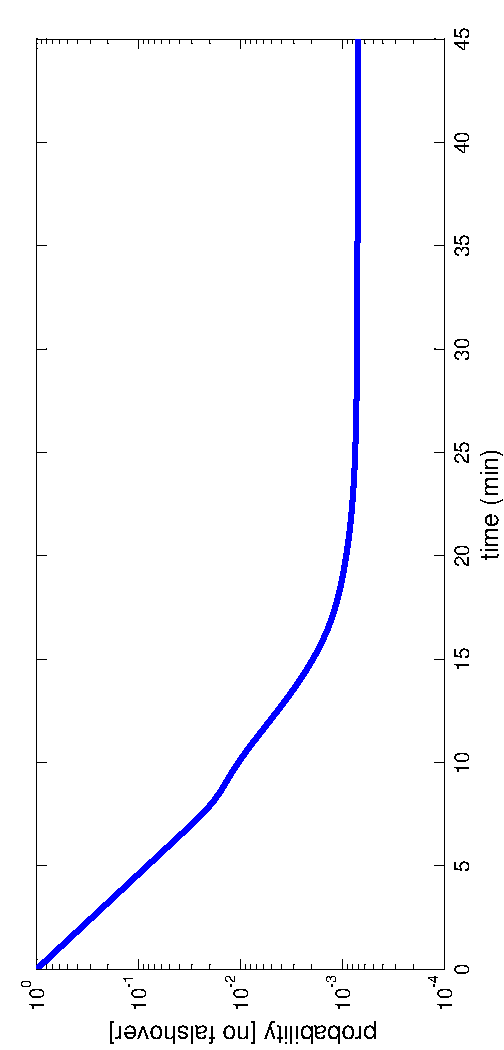
\includegraphics[scale=0.8, angle=-90]{NoFlashover}
  \caption{Probability that fire does not grow up to flashover.\label{fig:NoFlashover}} 
\end{figure}

Figure \ref{fig:NoFlashover} shows the sum $\sum_{i=2}^5 \phi_{2i}(t)$  of the probabilities of being in states other than non-fire and flashover. This represents the probability that fire is contained with in these four states without growing to a flashover. The probability starts with a certainty of 1 because ignition is the initial state and rapidly decreases from 100$\%$ to less than 1\% during early growth of fire. This reflects the immense potential of a flashover with in 15 to 20 minutes of ignition. Beyond this time, the possibility of a flashover or going to non-fire state has a steady probability of 93\%. This stability is due to the slowdown of fluctuation between the growing and receding fire. 
%%%%%%%%%%%%%%%%%%%%%%%%%%%%%%%%%%%%%%%%%%%%%%%%%%%%%%%%%%%%%%%%%%%%%%

\subsection{What if variability is ignored?}

Assume the case where all the distributions assumed in Table \ref{tbl:FireAssumedDists} are exponential $i.e,$ mean is the only parameter and the standard deviation is ignored. This case leads to a Markov process model and the resulting state probabilities are shown in Figure \ref{fig:FireStateProbsMarkov}. 

\begin{figure}[h!] \centering
  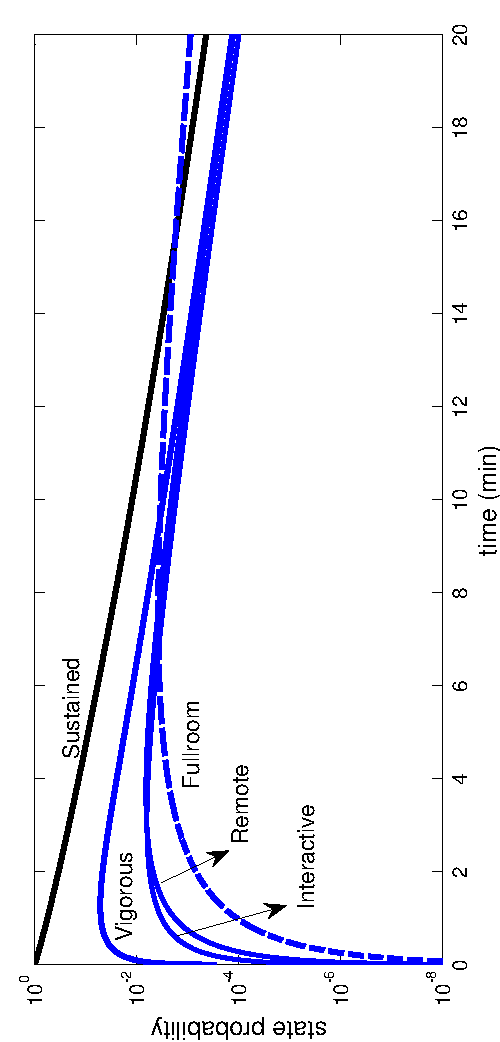
\includegraphics[scale=0.8, angle=-90]{FireStateProbsMarkov}
  \caption{Probability of being in each state.[Markov method]\label{fig:FireStateProbsMarkov}} 
\end{figure}


\begin{table}\centering
\caption{Time at which maximum state probabilities occur. [Markov method]\label{tbl:FireMaxProbsMarkov}}
\begin{tabular}{ l l l l}
	\hline
& State &	Maximum & Time (min) at which \\
&		& probability	(1)					&				 (1) occurs \\
	\hline
3 & Vigorous &		0.0516441	&	1.27	\\
4 & Interactive &   0.00627998 & 3.08	\\
5 & Remote & 0.00658725 & 3.71	\\
6 & Full room &    0.00376005 & 7.53	\\
  \hline
\end{tabular}
\end{table}

The overall trend compared to Figure \ref{fig:FireStateProbs} is similar though not identical. The striking difference can be seen from the time at which the maximum probabilities occur in Table \ref{tbl:FireMaxProbsMarkov}. For example, in the semi-Markov case, full-room involvement occurs at 15.3 minutes with maximum probability, the same happens at 7.53 minutes in the Markov case - less than half the time if variability is not considered. Similar observation is witnessed for the other states. Hence, assuming exponential distribution for all the state transitions could lead to potential misinterpretations through the Markov model.



%%%%%%%%%%%%%%%%%%%%%%%%%%%%%%%%%%%%%%%%%%%%%%%%%%%%%%%%%%%%%%%%%%%%%%
\section{Applications}
The proposed method as an early fire growth model has potential applications. Configuration of construction materials and detector devices are often different for residential and commercial buildings. Design considerations like the resistance of materials and response time of the devices can be influenced by running the proposed model with appropriate experimental test data. Building and fire codes are updated regularly based on changing requirements, new technologies and research outcomes. The proposed model can be used by fire safety regulators as a ``what if analysis'' tool. Sensitivity analysis can be done on the time needed to provide emergency fire services and mandatory requirements on the kind of material to be used in residential apartments and industrial sites.


%%%%%%%%%%%%%%%%%%%%%%%%%%%%%%%%%%%%%%%%%%%%%%%%%%%%%%%%%%%%%%%%%%%%%%
\section{Conclusions}
Existing fire behaviour models based on state transition methods were reviewed. An alternative and structured approach to fire growth modelling based on semi-Markov process model was proposed. The model has six states and takes in to account the ability to extinguish the fire.  The time dependent probability of being in each of the states based on existing experimental fire test data was determined. Interpretations were drawn based on the time at which maximum state probability occurred.  Further, the probability of the flame growth not reaching flashover or non-fire state was determined. The proposed model is useful to designers of construction materials and activation devices. The model can also be used by fire safety regulators to update safety standards.
%%%%%%%%%%%%%%%%%%%%%%%%%%%%%%%%%%%%%%%%%%%%%%%%%%%%%%%%%%%%%%%%%%%%%%
%%%%%%%%%%%%%%%%%%%%%%%%%%%%%%%%%%%%%%%%%%%%%%%%%%%%%%%%%%%%%%%%%%%%%%
% The bibliography is stored in an external database file
% in the BibTeX format (file_name.bib).  The bibliography is
% created by the following command and it will appear in this
% position in the document. You may, of course, create your
% own bibliography by using thebibliography environment as in
%
% \begin{thebibliography}{12}
% ...
% \bibitem{itemreference} D. E. Knudsen.
% {\em 1966 World Bnus Almanac.}
% {Permafrost Press, Novosibirsk.}
% ...
% \end{thebibliography}
% Here's where you specify the bibliography style file.
% The full file name for the bibliography style file 
% used for an ASME paper is asmems4.bst.
%\addcontentsline{toc}{section}{References}
\bibliographystyle{asmems4}
% Here's where you specify the bibliography database file.
% The full file name of the bibliography database for this
% article is asme2e.bib. The name for your database is up
% to you.
\bibliography{uw-ethesis}
%%%%%%%%%%%%%%%%%%%%%%%%%%%%%%%%%%%%%%%%%%%%%%%%%%%%%%%%%%%%%%%%%%%%%%


%%%%%%%%%%%%%%%%%%%%%%%%%%%%%%%%%%%%%%%%%%%%%%%%%%%%%%%%%%%%%%%%%%%%%%


\end{document}
